\section{Kartenerstellung}

Die ursprüngliche Idee unseres Projektes war folgende: Das Auto sollte einen unbekannten Rundkurs durchfahren und eine Karte der Strecke erstellen. Zur Unterstützung der Positionsbestimmung werden Marker plaziert, deren Position oder Abstand entlag der Strecke dem Auto bekannt oder unbekannt sind.
Nach der Durchfahrung könnte das Auto anhand der Karte eine Trajektorie zur Durchfahrung des Rundkurses berechnen, bei dem das Auto den Kurs in minimaler Zeit durchfährt und sich dabei gegebenenfalls noch an Verkehrsregeln wie zum Beispiel Geschwindigkeitsbegrenzungen hält, welche als Schilder von der Kamera des Autos wargenommen wurden.
Abschließend soll das Auto die berechnete Trajektorie abfahren.

Da der Umfang des Projektes ziemlich groß ist, haben wir uns fürs erste nur auf die Kartenerstellung eines unbekannten Rundkurses beschränkt und dabei verschiedene Verfahren getestet:

\subsection{Meilenstein 1 - Computersimulation}

Für unseren ersten Meilenstein wurde ein Kreis als unbekannte Strecke betrachtet. Mithilfe von Matlab und der Robotics Toolbox von Peter Corke sollte die Testfahrt simuliert werden und die Karte während der Durchfahrung durch das Erweiterte Kalman Filter bestimmt werden.
Dabei wurden für das Auto folgende Annahmen getroffen:
\begin{itemize}
 	\item Das Auto kennt die genaue Position der Marker
 	\item Bei jedem Berechnungsschritt stehen dem Auto fehlerbehaftete Odometriedaten (Geschwindigkeit und Lenkwinkel) zur Verfügung, wobei der Fehler normalverteilt ist und die Varianz bekannt ist
 	\item ist ein Marker im Sichtfeld der Kamera des Autos, so kann das Auto Abstand und Winkel zum Marker bestimmen. Diese Sensordaten sind auch mit einem normalverteilten Fehler behaftet, dessen Varianz bekannt ist.
\end{itemize}
Für die Simulation wurde ein "Driver" Objekt für die Robotics Toolbox implementiert, welches das Auto auf dem Kurs hält. Außerdem wurden einige Klassen modifiziert, damit beliebige Strecken und Anordnungen von Markern gewählt werden können.

Qualitativ beschrieben läuft die Simulation folgendermaßen ab:
Das Auto bewegt sich bei jedem Rechenschritt mit konstanter Geschwindigkeit und wird so gelenkt, dass es der Spur folgt. Gleichzeitig wird ein Prädiktionsschritt mit den Odometriedaten durchgeführt - die Orientierung des Autos und damit der Verlauf der Strecke wird durch Koppelnavigation (engl. dead reckoning) geschätzt.
Falls sich ein Marker im Sichtfeld des Autos befindet, wird zusätzlich noch ein Korrekturschritt ausgeführt. Dabei wird die Schätzung stärker korrigiert, je mehr die Sensordaten nicht zur erwarteten Orientierung passen. Nebenbei wird eine Kovarianzmatrix mitgeführt und aktualisiert, welche die Unsicherheit der Schätzung beschreibt.

In Abbildung~\ref{fig:simulation} sind die Simulationsergebnisse dargestellt.

\begin{figure}[h]
	\centering
    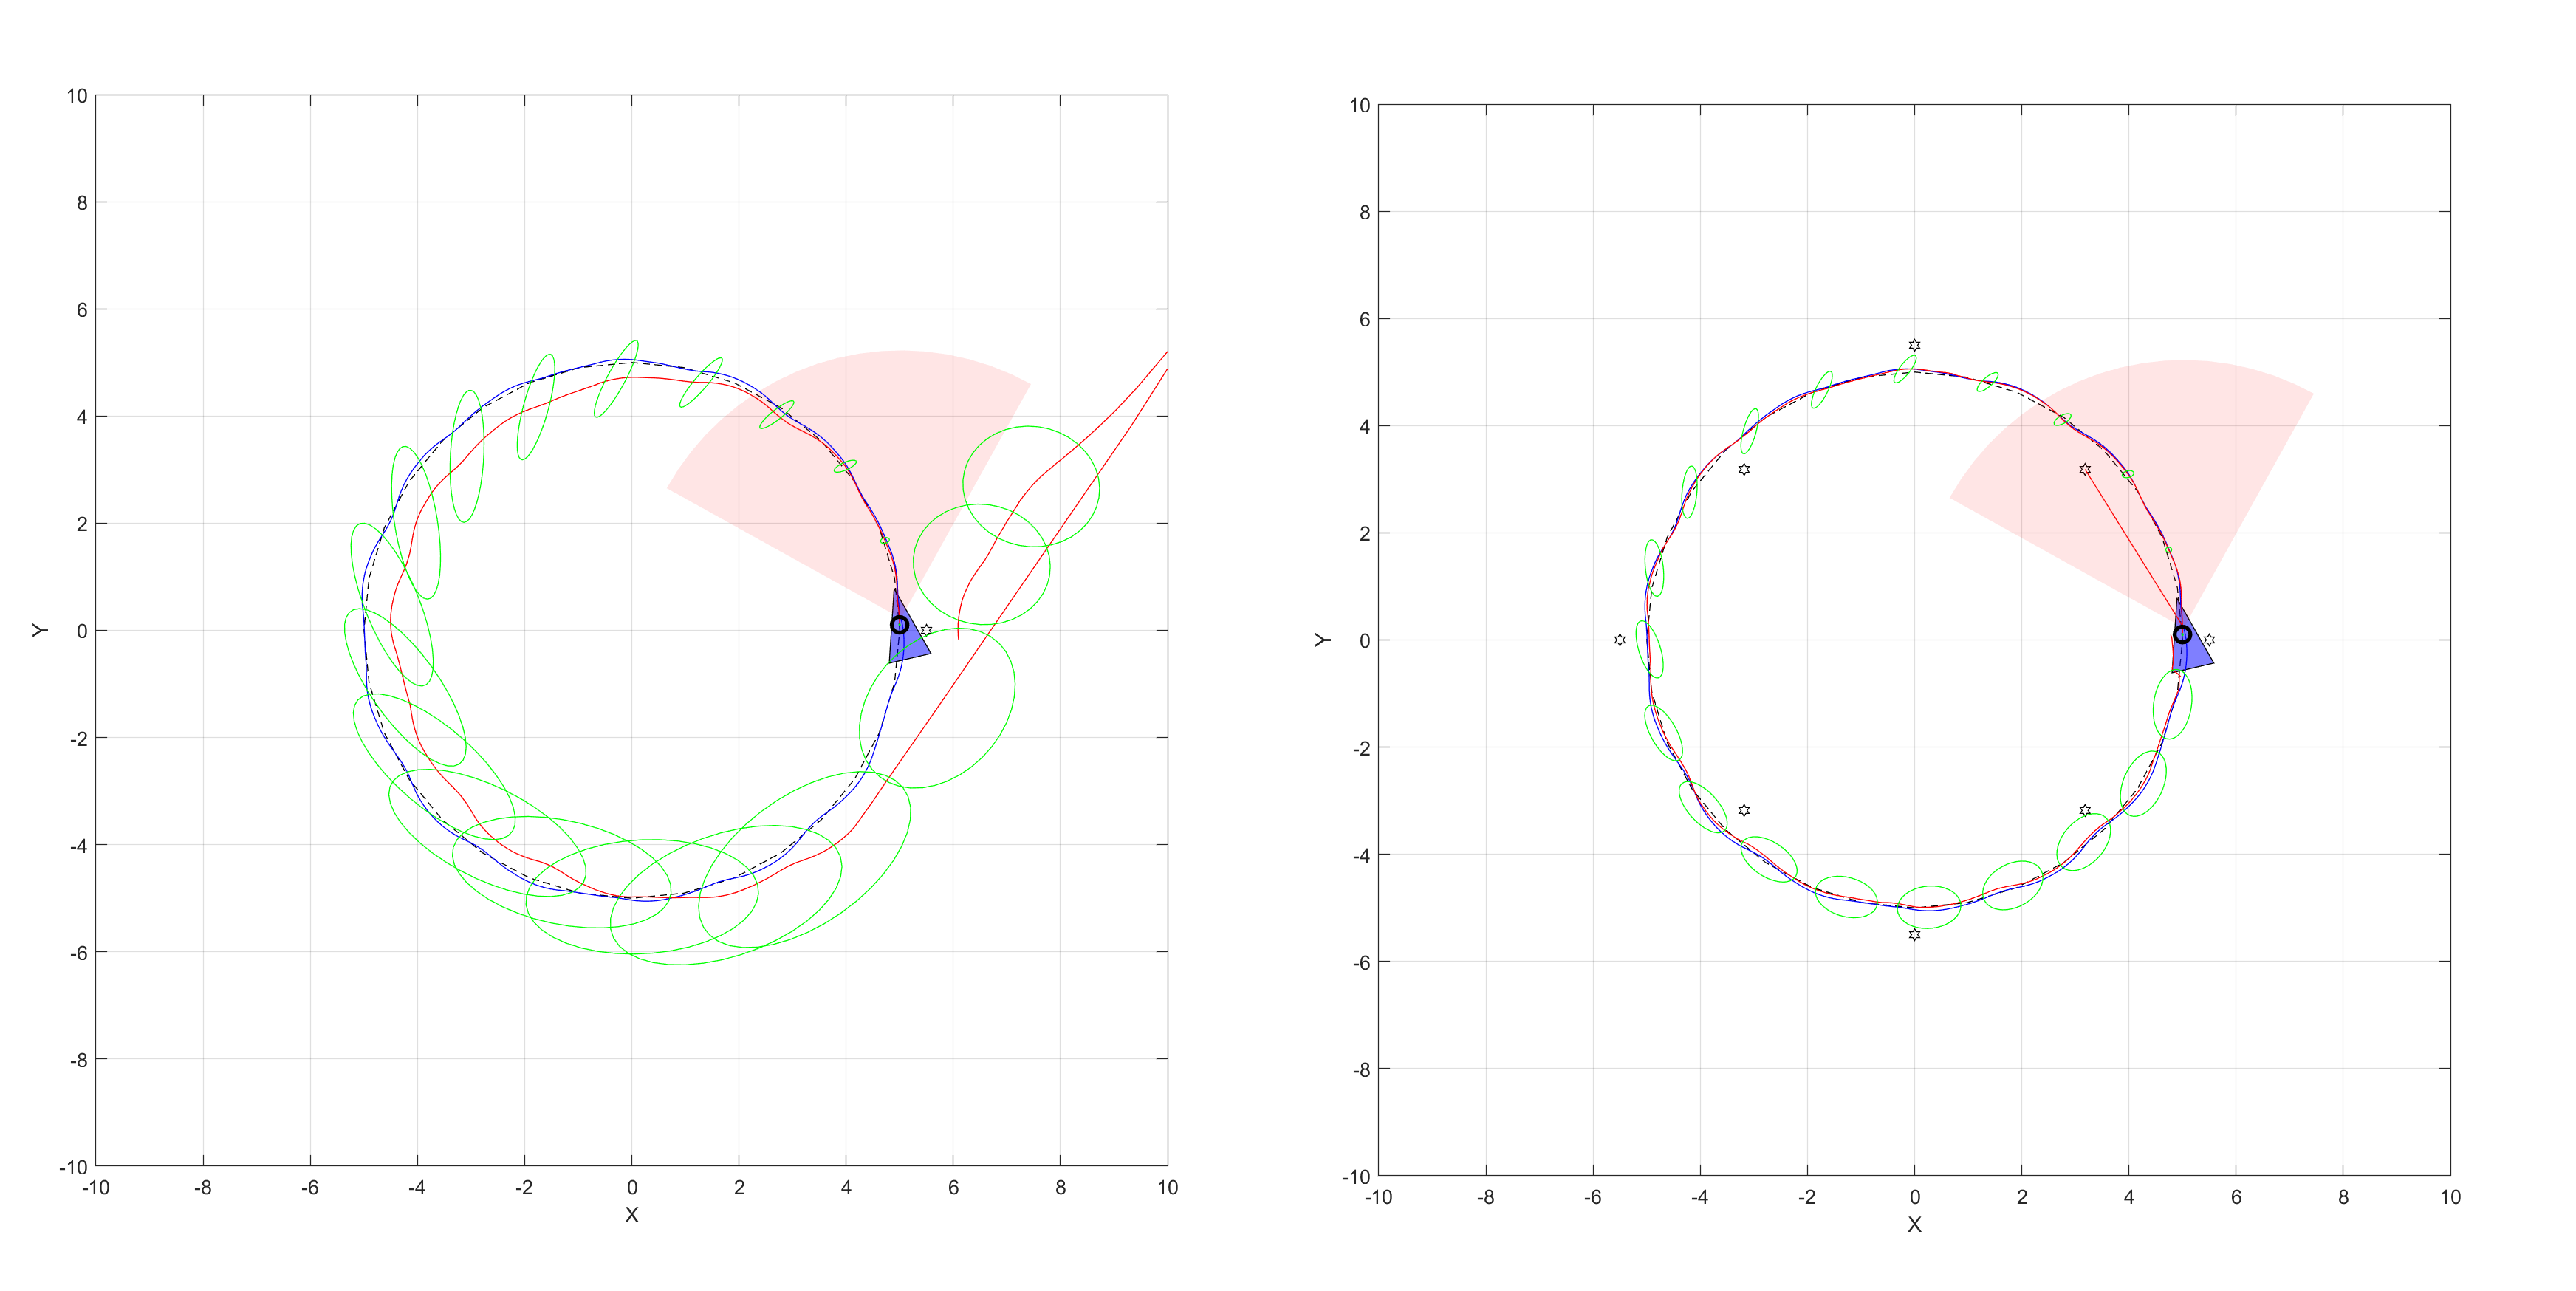
\includegraphics[width=.75\linewidth]{Figures/2.png}
	\caption{Kreisfahrt nur mit Startmarker und extra Markern. Die eigentlich gefahrene Strecke ist blau dargestellt, die geschätzte Strecke rot. Die grünen Ellipsen umranden den $1\sigma$ Bereich der Positionsunsicherheit}
	\label{fig:simulation}
\end{figure}

Schon nach Umfahrung des halben Kurses nur mit Startmarker ist eine deutliche Abweichung der geschätzten Strecke zur eigentlichen zu erkennen. Warum die geschätzte Position bei Erreichen des Startmarkers den Kartenbereich verlässt, bedarf noch eine genaurere Untersuchung.